\begin{quote}
	$$S=\set{x|x\notin x}$$
	
	\hfill --Georg Cantor

	Point set topology is a disease from which the human race will soon recover. Later generations will regard Mengenlehre (set theory) as a disease from which one has recovered.\hfill --Henri Poincare
	
	We are not speaking here of arbitrariness in any sense. Mathematics is not like a game whose tasks are determined by arbitrarily stipulated rules. Rather, it is a conceptual system possessing internal necessity that can only be so and by no means otherwise. \hfill --David Hilbert
\end{quote}

\section{简单的朴素集合论的一些定义}

在中学的时候, 我们定义的集合是如下的一个数学对象: \red{\bf 集合}就是任何一个\blue{有明确定义的}对象的\blue{整体}. 

\begin{definition}[集合]
    我们将\red{\bf 集合}理解为任何将\blue{我们思想中那些确定而彼此独立的对象}放在一起而形成的\blue{聚合}. 
\end{definition}

这也引出了概括原则: 

\begin{theorem}[概括原则]
    对于任意性质/谓词 $P(x)$, 都存在一个集合 $X$:
    \[
      X = \set{x \mid P(x)}
    \]
\end{theorem}

很多时候我们需要判别两个集合是不是相等, 那么我们有外延性原理: 
\begin{definition}[外延性原理 (Extensionality)]
    两个集合相等 $(A = B)$ 当且仅当它们包含相同的元素. 
    \[
      \forall A.\; \forall B.\;
        \Big(\big(\forall x.\; (x \in A \leftrightarrow x \in B)\big)
          \leftrightarrow A = B \Big)
    \]
\end{definition}

这条公理意味着集合这个对象完全由它的元素决定. 

有时候我们需要从一个集合里面抽出一部分, 也就是寻找一个集合的子集. 因此我们有如下的定义. 

\begin{definition}[子集]
    设 $A$、$B$ 是任意两个集合. 

    $A \subseteq B$ 表示 $A$ 是 $B$ 的\red{子集} (subset):
    \[
      A \subseteq B \iff \forall x \in A.\; (x \in A \to x \in B)
    \]

    $A \subset B$ 表示 $A$ 是 $B$ 的\red{真子集} (proper subset):
    \[
      A \subset B \iff A \subseteq B \land A \neq B
    \]
\end{definition}

我们还可以证明两个集合相等, 当二者互为对方的子集时候. 

\begin{theorem}
    两个集合相等当且仅当它们互为子集. 
    \[
      A = B \iff A \subseteq B \land B \subseteq A
    \]
\end{theorem}

然后, 让我们来对于高中学习过的操作重新定义一下. 

\begin{definition}[集合的并 (Union)]
    \[
      A \cup B \triangleq \set{ x \mid x \in A \lor x \in B}
    \]
\end{definition}

\begin{definition}[集合的交 (Intersection)]
    \[
      A \cap B \triangleq \set{x \mid x \in A \land x \in B}
    \]
\end{definition}

除此之外, 像命题逻辑一样, 集合也有一些运算的规律. 我们可以将它与命题逻辑一起观察, 并且发现其中的规律. 

\begin{theorem}[分配律 (Distributive Law)]
    \[
      A \cup (B \cap C) = (A \cup B) \cap (A \cup C)
    \]
    \[
      \teal{A \cap (B \cup C) = (A \cap B) \cup (A \cap C)}
    \]
\end{theorem}

对于这样的命题, 我们同样给出证明. 

\begin{proof}
    对任意$x$,
    \begin{align*}
        &x \in A \cup (B \cap C) \\
        \iff & (x \in A) \lor (x \in B \land x \in C) \\
        \red{\iff} & (x \in A \lor x \in B) \land (x \in A \lor x \in C) \\
        \iff & (x \in A \cup B) \land (x \in A \cup C) \\
        \iff & x \in (A \cup B) \cap (A \cup C)
      \end{align*}
\end{proof}

同样, 像命题符号一样, 集合的运算也遵循吸收率: 

\begin{theorem}[吸收律 (Absorption Law)]
    \[
      A \cup (A \cap B) = A
    \]
    \[
      \teal{A \cap (A \cup B) = A}
    \]
\end{theorem}

\begin{proof}
    对任意$x$,
    \begin{align*}
        &x \in A \cup (A \cap B) \\
        \iff & x \in A \lor (x \in A \land x \in B) \\
        \red{\iff} & x \in A
      \end{align*}
\end{proof}

有了这个我们就可以使用这个证明一个比较重要的习题. 

\begin{theorem}
    \[
      A \subseteq B \iff A \cup B = B \;\purple{\iff A \cap B = A}
    \]
  \end{theorem}
\begin{proof}
    
  对任意 $x$
    
  \setcounter{equation}{0}
  \begin{align*}
    &x \in B \\
    \red{\implies} &x \in A \lor x \in B \\
    \implies &x \in A \cup B
  \end{align*}
\end{proof}

\begin{definition}[集合的差 (Set Difference); \blue{相对补} (Relative Complement)]
  \[
    A \setminus B = \set{x \mid x \in A \land x \notin B}
  \]
\end{definition}

\begin{definition}[绝对补 (Absolute Complement); \purple{$\overline{A}, A', A^{c}$}]
  \red{设全集为$U$. }
  \[
    \overline{A} = U \setminus A = \set{x \in U \mid x \notin A}
  \]

  其中, 全集 $U$ (Universe) 是当前正在考虑的所有元素构成的集合. 一般均默认存在. 通常可以注意到: 不存在``包罗万象''的全集. 
\end{definition}


和命题逻辑一样, 相对补和绝对补之间就像是命题符号一样, 存在一些联系. 

\begin{theorem}[``相对补''与``绝对补''之间的关系]
  \red{设全集为 $U$. }
  \[
    \red{\boxed{A \setminus B = A \cap \overline{B}}}
  \]
\end{theorem}

\begin{proof}
  对任意 $x$,
  \setcounter{equation}{0}
  \begin{align*}
    &x \in A \setminus B \\
    \iff & x \in A \land x \notin B \\
    \red{\iff} & x \in A \land (x \in U \land x \notin B) \\
    \iff & x \in A \land x \in \overline{B} \\
    \iff & x \in A \cap \overline{B}
  \end{align*}
\end{proof}

\begin{theorem}[德摩根律 (绝对补)]
  \red{设全集为 $U$. }

  \[
    \overline{A \cup B} = \overline{A} \cap \overline{B}
  \]
  \[
    \teal{\overline{A \cap B} = \overline{A} \cup \overline{B}}
  \]
\end{theorem}
\begin{proof}
    对任意 $x$, 
  \setcounter{equation}{0}
  \begin{align*}
    &x \in \overline{A \cup B} \\
    \iff & x \in U \land \lnot (x \in A \lor x \in B) \\
    \red{\iff} & x \in U \land x \notin A \land x \notin B \\
    \iff & (x \in U \land x \notin A) \land (x \in U \land x \notin B) \\
    \iff & x \in \overline{A} \land x \in \overline{B} \\
    \iff & x \in \overline{A} \cap \overline{B}
  \end{align*}
\end{proof}

\begin{theorem}[德摩根律 (相对补)]
  \[
    C \setminus (A \cup B) = (C \setminus A) \cap (C \setminus B)
  \]
  \[
    \teal{C \setminus (A \cap B) = (C \setminus A) \cup (C \setminus B)}
  \]
\end{theorem}

\begin{proof}
  \setcounter{equation}{0}
  \begin{align*}
    &C \setminus (A \cup B) \\
    \red{\iff} & C \cap \overline{A \cup B} \\
    \iff & C \cap (\overline{A} \cap \overline{B}) \\
    \iff & (C \cap \overline{A}) \cap (C \cap \overline{B}) \\
    \iff & (C \setminus A) \cap (C \setminus B)
  \end{align*}
\end{proof}

这些命题的意义在于再证明集合相关的命题的时候, 就不需要从中抽出一个元素单独讨论了; 相反, 我们可以用集合整体的性质. 

\begin{proof}
  \setcounter{equation}{0}
  \begin{align*}
    &C \setminus (A \cup B) \\
    \red{\iff} & C \cap \overline{A \cup B} \\
    \iff & C \cap (\overline{A} \cap \overline{B}) \\
    \iff & (C \cap \overline{A}) \cap (C \cap \overline{B}) \\
    \iff & (C \setminus A) \cap (C \setminus B)
  \end{align*}
\end{proof}

这里面有一个类似一个异或操作的运算符: 对称差. 

\begin{definition}[对称差 (Symmetric Difference)]
  \[
    A \oplus B = (A \setminus B) \cup (B \setminus A)
      = (A \cap \overline{B}) \cup (B \cap \overline{A})
  \]
\end{definition}

\section{高级集合操作}
\subsection{交和并}

既然集合的对象是一组元素, 那么集合也是对象, 集合中的元素自然也可以被传进去看作运算. 由此, 我们需要定义关于集合的集合的运算. 

\begin{definition}[广义并 (Arbitrary Union)]
  设 $\mathbb{M}$ 是一组集合 (a {\it collection} of sets)
  \[
    \bigcup \mathbb{M} = \Bset{x \mid \red{\exists} A \in \mathbb{M}.\; x \in A}
  \]
\end{definition}

举一些例子, 比如$\mathbb{M} = \Bset{\set{1, 2}, \set{\set{1, 2}, 3}, \set{4, 5}}$, 那么$\bigcup \mathbb{M} = \Bset{1, 2, 3, 4, 5, \red{\set{1, 2}}}$. 注意元素只被解开了一次而不是一次解包到我们认为的``基本元素''. 因为有时候``基本元素''也是用集合定义的. 我们后来会发现我们可以把整个数学基础建立到集合论的基础上. 

和求和记号一样, 为了方便书写, 我们也有类似的记号: 
  \[
    \bigcup_{j = 1}^{n} A_j \triangleq A_1 \cup A_2 \cup \cdots \cup A_n
  \]
  \[
    \bigcup_{j = 1}^{\infty} A_j \triangleq A_1 \cup A_2 \cup \cdots
  \]
  \[
    \bigcup_{\blue{\alpha \in I}} A_{\alpha} \triangleq
      \Big\{x \mid \red{\exists} \alpha \in I.\; x \in A_{\alpha}\Big\}
  \]

和广义并一样, 我们还有广义交. 定义如下: 
\begin{definition}[广义交 (Arbitrary Intersection)]
  设 $\mathbb{M}$ 是一组集合 (a {\it collection} of sets)
  \[
    \bigcap \mathbb{M} = \Bset{x \mid \red{\forall} A \in \mathbb{M}.\; x \in A}
  \]
\end{definition}

同样的, 如果$\mathbb{M} = \Bset{\set{1, 2}, \set{\set{1, 2}, 3}, \set{4, 5}}$是全集,  $\bigcap \mathbb{M} = \emptyset$. 同样只是展开一次就行了. 注意一个有趣的情况: $\bigcap \emptyset =U$. ``包含所有元素的集合''在后面会发现会导出一个矛盾, 有时候我们也会认为这样说的结果是未定义的. 

那么类似的, 我们也希望广义集合里面有没有像普通集合的一些操作. 答案是肯定的. 下面我们来探讨一些有趣的内容. 

\begin{theorem}[德摩根律]
  \[
    X \setminus \bigcup_{\alpha \in I} A_{\alpha} = \bigcap_{\alpha \in I} (X \setminus A_{\alpha})
  \]

  \[
    \teal{X \setminus \bigcap_{\alpha \in I} A_{\alpha} = \bigcup_{\alpha \in I} (X \setminus A_{\alpha})}
  \]
\end{theorem}

\begin{proof}
  对任意 $x$,
  \setcounter{equation}{0}
  \begin{align*}
    &x \in X \setminus \bigcup_{\alpha \in I} A_{\alpha} \\
    \iff & x \in X \land \lnot(\exists \alpha \in I.\; x \in A_{\alpha}) \\
    \iff & x \in X \land (\forall \alpha \in I.\; x \notin A_{\alpha}) \\
    \red{\iff} & \forall \alpha \in I.\; (x \in X \land x \notin A_{\alpha}) \\
    \iff & x \in \bigcap_{\alpha \in I} (X \setminus A_{\alpha})
  \end{align*}
\end{proof}

我们同样可以用这条规律来化简集合, 而不用真正在一个集合的集合里面取出来一个元素. 

\begin{eg}
  如果
  \[
    X_n = \set{-n, -n+1, \cdots, 0, \cdots, n-1, n}
  \]
  请化简: 
  $$A = \mathbb{R} \setminus \bigcap_{n \in \mathbb{Z}^{+}} (\mathbb{R} \setminus X_n) $$
\end{eg}
\begin{proof}
  \begin{align*}
    A &= \mathbb{R} \setminus \bigcap_{n \in \mathbb{Z}^{+}} (\mathbb{R} \setminus X_n) \\
    &= \mathbb{R} \setminus \Big(\mathbb{R} \setminus \bigcup_{n \in \mathbb{Z}^{+}} X_n \Big) \\
    &= \mathbb{R} \setminus \Big(\mathbb{R} \setminus \mathbb{Z} \Big) \\
    &= \mathbb{Z}
  \end{align*}
\end{proof}

\subsection{排列的力量}

在高中, 我们学习了排列组合. 如果对于集合中的元素进行``选择性缺席'', 这样就可以让我们构造出更加复杂而全面的集合了. 

\begin{definition}[幂集 (Powerset)]
  \[
    \ps{A} = \Bset{X \mid X \subseteq A}
  \]
\end{definition}

这个之所以强大, 是因为给定一个$A$, 就有如下的内容可以被生成. 
  \[
    A = \set{1, 2, 3}
  \]
  \[
    \ps{A} = \set{\emptyset,
      \set{1}, \set{2}, \set{3},
      \set{1, 2}, \set{1, 3}, \set{2, 3},
      \set{1, 2, 3}}
  \]

因为对于$|A| = n$的句子, $|\ps{A}| = 2^{n}$, 因此有时候也写做$2^{A}$或者$\set{0,1}^{A}$. 

接下来看一个(看似)没啥用的定理: 

\begin{theorem}
  $$S \in \ps{X} \iff S \subseteq X$$
\end{theorem}

这个定理的作用是在$\in$和$\subseteq$之间转换, 同时脱去一层$\ps{}$记号. 

\begin{eg}
  请证明: 
  $$\set{\emptyset, \set{\emptyset}} \in \ps{\ps{\ps{S}}}$$
\end{eg}

\begin{proof}
  根据上面的定理, 我们有
  $$\set{\emptyset, \set{\emptyset}} \in \ps{\ps{\ps{S}}} \iff \set{\emptyset, \set{\emptyset}} \subseteq \ps{\ps{S}}.$$

  分别证明之: 
  \begin{align*}
    &\red{\emptyset \in \ps{\ps{S}}}\\
    &\iff \emptyset \subseteq \ps{S}
  \end{align*}

  \begin{align*}
    &\red{\set{\emptyset} \in \ps{\ps{S}}}\\
    &\iff \set{\emptyset} \subseteq \ps{S}\\
    &\iff \emptyset \in \ps{S}\\
    &\iff \emptyset \subseteq S
  \end{align*}

\end{proof}

其实幂集生成之间也有一些关系. 不妨看一看. 

\begin{theorem}
  证明: 
  \[
      \ps{A} \cap \ps{B} = \ps{A \cap B}
  \]
\end{theorem}

\begin{proof}
  对于任意 $x$,
  \begin{align*}
    &\textcolor{white}{\iff}\;\; x \in \ps{A} \cap \ps{B} \\
    &\iff x \in \ps{A} \land x \in \ps{B} \\
    &\iff x \subseteq A \land x \subseteq B \\
    &\iff x \subseteq A \cap B \\
    &\iff x \in \ps{A \cap B}
  \end{align*}
\end{proof}

\begin{theorem}
  证明: 
  \[
    \bigcap_{\alpha \in I} \ps{A_{\alpha}} = \ps{\bigcap_{\alpha \in I} A_{\alpha}}
  \]
\end{theorem}

\begin{proof}
  对于任意 $x$,
  \begin{align*}
    &\textcolor{white}{\iff}\;\; x \in \bigcap_{\alpha \in I} \ps{A_{\alpha}} \\
    &\iff \forall \alpha \in I.\; x \in \ps{A_{\alpha}} \\
    &\iff \forall \alpha \in I.\; x \subseteq A_{\alpha} \\
    &\iff x \subseteq \bigcap_{\alpha \in I} A_{\alpha} \\
    &\iff x \in \ps{\bigcap_{\alpha \in I} A_{\alpha}}
  \end{align*}
\end{proof}

\section{悖论的出现}

前面我们提到``不存在含有任何东西的集合''. 这就是我们以前知道的通俗讲述的``理发师悖论''. 形式化的, 根据概括原则, 如果性质$P$是$P(x) \triangleq ``x \notin x"$, 集合$R = \set{x \mid x \notin x}$, 那么$R \in R\;$吗? 

\begin{quote}
  ``悖论出现于数学的边界上, 而且是靠近哲学的边界上''
  \hfill --- Godel
\end{quote}

之后, 数学家们提出了ZF(ZFC)公理化集合论, 避免了这样的内容. 通过粗暴的避免了这种情况, 我们得到了一个还可以使用, 但是丧失了一部分确定性的集合. 


\section{二元关系: 简介以及简单运算}

我们在初中和高中的学习中学习了很多的``关系''. 比如, 比较两个数的大小, 我们引入了``大于'', ``小于''和``等于''的关系. 这样的内容我们可以进一步的抽象, 提炼出``关系''的一些共性. 

比如, 我们可以在$\R$上定义``Near''关系.

\begin{eg}
    如果$|a - b| < 1(a, b \in \R)$, 则称$a, b$具有Near关系. 
\end{eg}

回顾我们学过的表达``关系''的运算符, 相当一部分满足下面的性质: 

\textbf{自反性. }
$$\forall a \in X.\; (a, a) \in R$$

\textbf{对称性. }
$$\forall a, b \in X.\; ((a, b) \in R \to (b, a) \in R)$$

\textbf{传递性. }
$$\forall a, b, c \in X.\; ((a, b) \in R \land (b, c) \in R \to (a, c) \in R)$$

很多时候, 我们把自反性 + 对称性 = 相容关系. 相容关系的含义其实是表明这两个关系之间有交叉.

这样, 我们就可以把关系表示成一个集合. 不严格的说, 在上面的定义中, 我们可以有这样的集合: $R = \set{(a, b) \mid |a - b| < 1}$. 

下面来看几个更多的例子. 比如整除关系. 

\begin{eg}
    假设$X = \set{1, 2, 3, 4, 5, 6, 10, 12, 15, 20, 30, 60}$, ``关系''是$X$ 上的整除关系. 
\end{eg}

按照上面的展开, 我们就有所有整除的全体(有序对$(a,b)$表示的关系是$a|b$):
$$R = \set{(1, 2), \dots, (4, 12), \dots, (12, 60), \dots, (4, 60), \dots, (60, 60)}$$

可以看到在上述的关系中, 上面的自反性, 对称性, 传递性仍然满足. 这种结构十分的常见. 比如地图上面的地方的``可达''关系, 还有给定集合的幂集按``包含''关系排序, 自然数按照大小关系排序, 等等. 满足上述的三条性质的关系叫做``偏序关系''. 特殊的, 我们或许还会发现自然数可以唯一地按照大小被排成一排, 这是一种比较特殊的偏序关系, 后来我们会定义它为全序关系. 

特别的, 我们可以把上述偏序关系画成一张图, 也就是在多个维度上都有不同的序, 因此没办法唯一的列成一列, 包含所有元素. 

比如上述的幂集的例子, 化作一张图\ref{fig:part-order-fig}所示: 
\begin{figure}[!htbp]
	\begin{center}
	    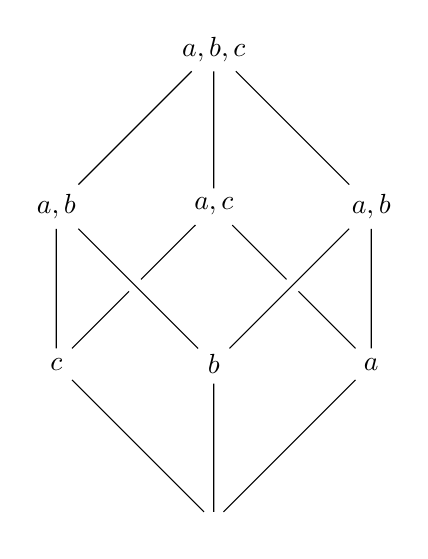
\begin{tikzpicture}
    	\node (max) at (0,4) {$\set{a,b,c}$};
    	\node (a) at (-2,2) {$\set{a,b}$};
  		\node (b) at (0,2) {$\set{a,c}$};
    	\node (c) at (2,2) {$\set{a,b}$};
    	\node (d) at (-2,0) {$\set{c}$};
    	\node (e) at (0,0) {$\set{b}$};
    	\node (f) at (2,0) {$\set{a}$};
    	\node (min) at (0,-2) {$\set{}$};
    	\draw (min) -- (d) -- (a) -- (max) -- (b) -- (f)
    (e) -- (min) -- (f) -- (c) -- (max)
    (d) -- (b);
    	\draw[preaction={draw=white, -,line width=6pt}] (a) -- (e) -- (c);
 	\end{tikzpicture}
	\end{center}
	\caption{偏序关系的图示}
	\label{fig:part-order-fig}
\end{figure}

观察正整数集, 发现这是一条链式结构, 它和上述的偏序集最大的区别是什么呢? 其实, 最大的区别是在整数中的大于关系存在``连接性''. 

\textbf{连接性.} 
$$
\forall a, b \in X.\; ((a, b) \in R \lor (b, a) \in R)
$$

也就是自反性 + 反对称性 + 传递性 + 连接性 = \red{\bf 全序关系}. 

\subsection{有序对}

我们可能会很自然的想$ (a, b) = (c, d) \iff a = c \land b = d$, 对于这样自然产生的概念, 我们同样要将它严格化, 给出一个定义.  

历史上, 很多人会用集合的观念来刻画有序对. Norbert Wiener在1914年给出了这样的定义. 

\begin{definition}[Ordered Pairs \teal{(Norbert Wiener; 1914)}]
    \[
      (a, b) \;\red{\triangleq}\; \Bset{\bset{\set{a}, \emptyset}, \bset{\set{b}}}
    \]
\end{definition}

这样一来, 有序对之间的相等关系看上去就自然了很多. 

\begin{theorem}
    \[
      (a, b) = (c, d) \iff a = c \land b = d
    \]
\end{theorem}
\begin{proof}
    也就是证明
    $$\Big(\bset{\set{a}, \set{a, b}} = \bset{\set{c}, \set{c, d}}\Big) \iff (a = c \land b = d)$$
    我们有: 
    \begin{align*}
        &\bset{\set{a}, \set{a, b}} = \bset{\set{c}, \set{c, d}} \\
        \iff& (\set{a} = \set{c} \lor \set{a} = \set{c, d}) \land (\set{a, b} = \set{c} \lor \set{a, b} = \set{c, d}) \\
        \iff& (\set{a} = \set{c} \land \set{a, b} = \set{c}) \;\lor \\
                         & (\set{a} = \set{c} \land \set{a, b} = \set{c, d}) \;\lor \\
                         & (\set{a} = \set{c, d} \land \set{a, b} = \set{c}) \;\lor \\
                         & (\set{a} = \set{c, d} \land \set{a, b} = \set{c, d})
      \end{align*}
    

\end{proof}

有了有序对, 我们还可以把它拓广到$n$个元素的情况. 于是我们有定义: 

\begin{definition}[$n$-元组 (n-ary tuples)]
    \[
      (x, y, z) \triangleq ((x, y), z)
    \]
    \[
      (x_{1}, x_{2}, \dots, x_{n-1}, x_{n})
        \triangleq ((x_{1}, x_{2}, \dots, x_{n-1}), x_{n})
    \]
\end{definition}

在这个结构上同样是可以应用数学归纳法的. 不过一般我处理而二元组就行了. 多数情况下, 我们仅处理``二元关系'', 因此也仅使用``有序对''

\subsection{笛卡尔积: 一种组合方式}

如果我们有两个集合, 从两个集合中各取得一个元素, 把它们组合成一个有序对,塞到一个新的集合里面, 这样, 我们就可以对于集合做一点组合, 生成更加复杂的集合了. 这样的操作叫做笛卡尔积.  

\begin{definition}[笛卡尔积 (Cartesian Products)]
    The \red{\it Cartesian product} $A \times B$ \blue{of $A$ and $B$}
    is defined as
    \[
      {A \times B \triangleq \set{(a, b) \mid a \in A \land b \in B}}
    \]
\end{definition}

那么``笛卡尔积''这个操作满足哪些运算律呢? 我们首先来考察一些例子. 

\begin{eg}
  
  \begin{align*}
  X\times \emptyset = \emptyset \times X \\
  X\times Y \neq  Y \times X \\
  (X \times Y) \times Z \;\neq\; X \times (Y \times Z)\\
  A = \set{1} \qquad (A \times A) \times A \;\red{\neq}\; A \times (A \times A)
  \end{align*}
  
\end{eg}

我们发现这个符号既没有普遍的交换律, 也没有普遍的结合律. 但是是有分配律的. 

\begin{theorem}[分配律 (Distributivity)]
  \[
    A \times (B \cap C) = (A \times B) \cap (A \times C)
  \]
  \[
    A \times (B \cup C) = (A \times B) \cup (A \times C)
  \]
  \[
    A \times (B \setminus C) = (A \times B) \setminus (A \times C)
  \]
\end{theorem}

下面我们来以证明$A \times (B \cap C) = (A \times B) \cap (A \times C)$为例, 看一下这个是如何进行起作用的. 
\begin{proof}
  \red{对任意\blue{有序对} $(a, b)$,}
    \setcounter{equation}{0}
    \begin{align*}
      &(a, b) \in A \times (B \cap C) \\
      \iff& a \in A \land b \in (B \cap C) \\
      \iff& a \in A \land b \in B \land b \in C \\
      \iff& (\blue{a \in A} \land b \in B) \land (\blue{a \in A} \land b \in C) \\
      \iff& (a, b) \in A \times B \land (a, b) \in A \times C \\
      \iff& (a, b) \in (A \times B) \cap (A \times C)
  \end{align*}
\end{proof}

同样的, 我们可以有多个元素的笛卡尔积. 

\begin{definition}[$n$-元笛卡尔积 ($n$-ary Cartesian Product)]
  \[
    X_{1} \times X_{2} \times X_{3} \triangleq (X_{1} \times X_{2}) \times X_{3}
  \]
  \[
    X_{1} \times X_{2} \times \dots \times X_{n}
      \triangleq (X_{1} \times X_{2} \times \dots \times X_{n-1}) \times X_{n}
  \]
\end{definition}

回想我们从数轴到平面直角坐标系再到空间直角坐标系, 我们可以发现这样的过程也就是对于一个维度反复做笛卡尔积的结果. 

但在本节的情况下, 我们仅处理``二元关系'', 因此也仅使用``二元笛卡尔积''. 


\subsection{用有序对定义二元关系}

我们以前做了有关关系的定义, 但是我们可能还要给``什么是关系''在集合方面下一个稍微集合化的定义. 于是我们有定义: 
\begin{definition}[关系 (Relations)]
  A \red{\it relation} $R$ \blue{from $A$ to $B$}
  is a \teal{subset} of $A \times B$:
  \[
    {R \subseteq A \times B}
  \]
  Sepcially,{align*} if $A = B$, $R$ is called a relation \blue{on} $A$.
\end{definition}

为了简化符号, 我们有时候也通过这样的方式来书写: 

\begin{definition}[Notations]
  \[
    (a, b) \in R \qquad a R b
  \]
  \[
    (a, b) \notin R \qquad a \overline{R} b
  \]
\end{definition}

举一些例子: $A\times B$ 和 $\emptyset$ 都是从 $A$ 到 $B$ 的关系, 前者的意义是任意两个$A$和$B$中的元素都有关系, 后者是都没有关系. 回顾我们在小学中学更一般的关系, 我们就会发现有更加有趣的二元关系: 
\begin{itemize}
  \item 小于关系: $<\; = \set{(a, b) \in \mathbb{R} \times \mathbb{R} \mid a \text{ is less than } b}$
  \item 整除关系: $D = \set{(a, b) \in \mathbb{N} \times \mathbb{N} \mid \exists q \in \mathbb{N}.\; a \cdot q = b}$
\end{itemize}

在生活中更有这样的关系. 比如$P$是所有人的集合, 如果我们定义$\red{M} = \set{(a, b) \in P \times P \mid a \text{ is the mother of } b}$, $\red{B} = \set{(a, b) \in P \times P \mid a \text{ is the brother of } b}$, 那么上述定义的$M$和$B$都满足``关系''的定义.

有了这样的抽象, 我们就可以很开心的研究另外一些更重要的问题了. 具体地, 我们要研究这些重要的关系: 
\begin{itemize}
  \item 等价关系
  \item 序关系
  \item 函数
\end{itemize}


\subsection{关系的简单运算}

在进行之前, 我们认为对于关系的运算进行一些内容. 

总体而言, 在这一小节中我们会给出三个定义, 5个操作, 以及7个对应的性质. 

其实, 这一节的内容很大程度上和中学定义的函数类似. 但是有一个重大的区别. 从现在开始, 我们稍微忘记我们高中关于``函数''的定义, 但是留下``函数''带给我们的思考方式. 下面我们来用有序对重新解释这一切. 

\ti{三个定义}

\begin{definition}[定义域 (Domain)]
  \[
    \text{dom}(R) = \set{a \mid \exists b.\; (a,b) \in R}
  \]
\end{definition}

我们在函数中说``定义域''是函数中有定义的地方的横坐标构成的集合, 在这里面的$\exists b$就保证了在这个点一定被定义了, 那么我们就取出来它的$a$(横坐标). ``扫描''所有这样的有序对$(a,b)$并将满足条件的$a$取出来, 我们就完成了这样类似概念的迁移. 

\begin{definition}[值域 (Range)]
  \[
    \text{ran}(R) = \set{b \mid \exists a.\; (a,b) \in R}
  \]
\end{definition}

我们在函数中说``值域''是函数中所有有定义的横坐标所对应的纵坐标, 在这里面的$\exists a$就说明了有这样的点被取到, 那么我们就取出来它的$b$(横坐标). ``扫描''所有这样的有序对$(a,b)$并将满足条件的$b$取出来, 同样有类似的概念. 

\begin{definition}[域 (Field)]
  \[
    \text{fld}(R) = \text{dom}(R) \cup \text{ran}(R)
  \]
\end{definition}

定义域和值域并起来就是域. 这样可以让我们直观的明确了解``二元关系''之间的空间映射关系. 

举个例子: 对于$R = \set{(x, y) \mid x^2 + y^2 = 1} \subseteq \R \times \R$, 它的$\dom(R) = [1, 1]$, $\ran(R) = [-1, 1]$, $\fld(R) = [-1, 1]$. 

我们来看一个更抽象的. 不过别忘了本质上就是用集合的操作解决这一切问题. 

\begin{theorem}
  \[
    \dom(R) \subseteq \bigcup \bigcup R \qquad
    \ran(R) \subseteq \bigcup \bigcup R
  \]
\end{theorem}

\begin{proof}
  \red{对任意 $a$,}
    \begin{align*}
      &a \in \dom(R) \\
      \implies& \exists b.\; (a, b) \in R \\
      \implies& \exists b.\; \blue{\set{\set{a}, \set{a, b}}} \in R \\
      \implies& \exists b.\; \set{a, b} \in \bigcup R \\
      \implies& \exists b.\; a \in \bigcup\bigcup R \\
      \implies& a \in \bigcup\bigcup R
    \end{align*}
\end{proof}

这个例子的直观解释就是任何的定义域, 值域都会在二元组的某一个元素中``出现''. 

\ti{五种操作}

\textbf{1. 逆变换. }像``反函数''的概念一样, 关系有时候也有逆变换. 

\begin{definition}[逆 (Inverse)]
  The {\it inverse} of $R$ is the \purple{relation}
  \[
    R^{-1} = \set{(a, b) \mid (b, a) \in R}
  \]
\end{definition}

我们可以来看几组例子: 
\begin{itemize}
  \item 如果$R = \set{(x, y) \mid x = y}\subseteq \R \times \R$, $R^{-1} = R$
  \item $R = \set{(x, y) \mid y = \sqrt{x}} \subseteq \R \times \R$, $R^{-1} = \set{(x, y) \mid y = x^{2} \land x > 0}$
  \item $\le = \set{(x, y) \mid x \le y} \subseteq \R \times \R \qquad$, $\le^{-1} \;= \ge \;\triangleq \set{(x, y) \mid x \ge y}$
\end{itemize}

直观地, 我们自然会想到反关系的反仍然是原来的关系. 所以我们有如下定理: 

\begin{theorem}
  \[
    (R^{-1})^{-1} = R
  \]
\end{theorem}

\begin{proof}
  \red{对任意 $(a, b)$,}
  \setcounter{equation}{0}
  \begin{align*}
    &(a, b) \in (R^{-1})^{-1} \\
    \iff& (b, a) \in R^{-1} \\
    \iff& (a, b) \in R
  \end{align*}
\end{proof}

既然关系也是集合定义的, 那我们自然可以证明它的交, 并, 补. 在我们做的有益的探索中, 我们会发现这个定理还是比较重要的. 

\begin{theorem}[关系的逆]
    如果$R, S$ 均为关系, 那么有
  \[
    (R \cup S)^{-1} = R^{-1} \cup S^{-1}
  \]
  \[
    (R \cap S)^{-1} = R^{-1} \cap S^{-1}
  \]
  \[
    (R \setminus S)^{-1} = R^{-1} \setminus S^{-1}
  \]
\end{theorem}

\textbf{2. 限制. } 由于问题的定义和性质, 有时候我们可能需要对于构造的``全面''集合的状态空间进行``裁切'', 来打造更精细的集合. 这样就可以自然地引入集合的限制操作. 我们希望引入这样的记号, 使得它可以对于这个关系二元组$(a,b)$中的$a$, $b$分别加以筛选. 于是我们有定义: 

\begin{definition}[左限制 (Left-Restriction)]
  Suppose $R \subseteq X \times Y$ and $S \subseteq X$.
  The {\it left-restriction} relation of $R$ \blue{to $S$} over $X$ and $Y$ is
  \[
    R|_{S} = \set{(x, y) \in R \mid \red{x \in S}}
  \]
\end{definition}

\begin{definition}[右限制 (Right-Restriction)]
  Suppose $R \subseteq X \times Y$ and $S \subseteq Y$.
  The {\it right-restriction} relation of $R$ \blue{to $S$} over $X$ and $Y$ is
  \[
    R|^{S} = \set{(x, y) \in R \mid \red{y \in S}}
  \]
\end{definition}

\begin{definition}[限制 (Restriction)]
  Suppose $R \subseteq X \times X$ and $S \subseteq X$.
  The {\it restriction} relation of $R$ \blue{to $S$} over $X$ is
  \[
    R|_{S} = \set{(x, y) \in R \mid \red{x \in S \land y \in S}}
  \]
\end{definition}

哎呀! ``限制''和``左限制''的记号重复了! 但是仔细看一下他们的前提是不一样的. ``左限制''的前提是有$R \subseteq X \times X$, 而``限制''的前提是$R \subseteq X \times X$, 也就是自己集合中元素到自己集合元素的关系. 

下面我们来看刚刚举的例子: 如果$R = \set{(x, y) \mid x^2 + y^2 = 1} \subseteq \R \times \R$, $R|_{\R^{+}}$的含义就是表示关系的二元组$(a,b)中$, $a$只取$\R^+$的时候满足的才被认为``满足''关系. 

\begin{bonus}
对于这样的情况, 我们能不能使用$xOy$平面表达这种关系呢? 限制在平面上的意义是什么? 
\end{bonus}

\vspace*{1pt}
\textbf{3. 像(Image). } 想一想这种``有所对应''的感觉, 好像在高中学习函数那一节里面见过类似的, 也就是有点像函数里面$f()$做的事情.  同样的, 这里面也有类似描述这样一种``有所对应''的定义. 

\begin{definition}[像 (Image)]
  The {\it image} of $X$ \blue{under $R$} is the set
  \[
    R[X] = \set{\red{b \in \text{ran}(R)} \mid \exists a \in X.\; (a, b) \in R}
  \]
\end{definition}
为了简化符号, 一般而言$R[a] \triangleq R[\set{a}] = \set{b \mid (a, b) \in R}$. 


\textbf{4.逆像. } 同样的, 我们有时候可能需要顺藤摸瓜, 这就自然地导出了像也有``逆''的概念. 

\begin{definition}[逆像 (Inverse Image)]
  The {\it inverse image} of $Y$ \blue{under $R$} is the set
  \[
    R^{-1}[Y] = \set{\red{a \in \text{dom}(R)} \mid \exists b \in Y.\; (a, b) \in R}
  \]
\end{definition}
同样为了简化记号, 我们有$R^{-1}[b] \triangleq R^{-1}[\set{b}] = \set{a \mid (a, b) \in R}$. 

有了这两个操作之后, 事情就变得复杂了. 比如$R^{-1}[R[X]] $和$ X$的关系如何, $R[R^{-1}[Y]]$和$Y$的关系又如何? 经过证明, 我们给出如下的定理: 
  
\begin{theorem}
  \[
    R[X_1 \cup X_2] = R[X_1] \cup R[X_2]
  \]
  \[
    R[X_1 \cap X_2] \subseteq R[X_1] \cap R[X_2]
  \]
  \[
    \teal{R[X_1 \setminus X_2] \supseteq R[X_1] \setminus R[X_2]}
  \]
\end{theorem}
\begin{proof}
  \red{对任意 $(a, b)$,}
  \setcounter{equation}{0}
  \begin{align*}
    &(a, b) \in (R \circ S)^{-1} \\
    \iff& (b, a) \in R \circ S \\
    \iff& \exists c.\; (b, \blue{c}) \in S \land (\blue{c}, a) \in R \\
    \iff& \exists c.\; (\purple{c}, b) \in S^{-1} \land (a, \purple{c}) \in R^{-1} \\
    \iff& (a, b) \in S^{-1} \circ R^{-1}
  \end{align*}
\end{proof}
\begin{theorem}
  \[
    (R \circ S) \circ T = R \circ (S \circ T)
  \]
\end{theorem}

\textbf{5. 复合. } 像复合函数一样, 这是一种构建复杂系统的很好的一种方法. 因此我们自然给出定义: 
\begin{definition}[复合 (Composition; $R \circ S$, $R ; S$)]
  The {\it composition} of relations $R \subseteq X \times \blue{Y}$
  and $S \subseteq \blue{Y} \times Z$ is the \purple{relation}
  \[
    R \circ S = \set{(a, c) \mid \exists b.\; (a, \blue{b}) \in S \land (\blue{b}, c) \in R}
  \]
\end{definition}

举个例子, $R = \set{(1, 2), (3, 1)} \qquad S = \set{(1, 3), (2, 2), (2, 3)}$, 那么$R \circ S = \set{(1, 1), (2, 1)}$, $S \circ R = \set{(1, 2), (1, 3), (3, 3)}$. 因为这个和``乘法''比较相似, 有时候我们也用空心圆圈表示. $R^{(2)} \triangleq R \circ R = \set{(3, 2)}$, $ (R \circ R) \circ R =  \emptyset$. 

\begin{bonus}
  有的人习惯记号$A\circ B\circ C=A\circ (B\circ C)$, 还有的人习惯$A\circ B\circ C=(A\circ B)\circ C$. 这样做有区别吗?  
\end{bonus}
\begin{theorem}
  \[
    (R \circ S) \circ T = R \circ (S \circ T)
  \]
\end{theorem}
\begin{proof}
  \red{对任意 $(a, b)$,}
  \setcounter{equation}{0}
  \begin{align*}
    &(a, b) \in (R \circ S) \circ T \\
    \iff& \exists c.\; \Big((a, c) \in T \land (c, b) \in R \circ S\Big) \\
    \iff& \exists c.\; \Big((a, c) \in T \land \red{\big(}\exists d.\; (c, d) \in S \land (d, b) \in R\red{\big)}\Big) \\
    \red{\iff}& \exists d.\; \exists c.\; \Big((a, c) \in T \land (c, d) \in S \land (d, b) \in R\Big) \\
    \iff& \exists d.\; \Big(\red{\big(}\exists c.\; (a, c) \in T \land (c, d) \in S\red{\big)} \land (d, b) \in R\Big) \\
    \iff& \exists d.\; \Big((a, d) \in S \circ T \land (d, b) \in R\Big) \\
    \iff& (a, b) \in R \circ (S \circ T)
  \end{align*} 
\end{proof}

这就表明关系的复合满足结合律, 但是不满足交换律(和矩阵乘法很相似). 
\ti{七个性质}

\textbf{1. 自反的. }

\begin{definition}[自反的 (Reflexive)]
  $R \subseteq X \times X$ is \red{\it reflexive} if
  \[
    \forall a \in X.\; (a, a) \in R
  \]
  \begin{center}
\begin{tikzpicture}
    \node[state] (s0) {$a$};
    \draw(s0) edge[loop above] (s0);
\end{tikzpicture}
\end{center}\end{definition}

举几个例子: 
\begin{itemize}
  \item $\le \;\subseteq \R \times \R \text{ is reflexive}$
  \item $\text{三角形上的\red{全等关系}是自反的}$
\end{itemize}

其实所有自反的关系都是这个关系的一个子集, 可以有如下的表达. 

\begin{theorem}
  \[
    R \text{ is reflexive} \iff I \subseteq R
  \]
  其中
  $$I = \set{(a, a) \in A \times A \mid a \in A}.$$
\end{theorem}

\begin{theorem}
  \[R \text{is reflexive} \iff R^{-1}=R\]
\end{theorem}


\textbf{2. 反自反. }

\begin{definition}[反自反 (Irreflexive)]
  $R \subseteq X \times X$ is \red{\it irreflexive} if
  \[
    \forall a \in X.\; (a, a) \notin R
  \]
\end{definition}

同样的, 我们给一些例子: 
\begin{itemize}
  \item $< \;\subseteq \R \times \R \text{ is irreflexive}$
  \item $> \;\subseteq \R \times \R \text{ is irreflexive}$
\end{itemize}

\textbf{3. 对称. }

\begin{definition}[对称 (Symmetric)]
  $R \subseteq X \times X$ is \red{\it symmetric} if
  \[
    \forall a, b \in X.\; a R b \to b R a
  \]

  \begin{center}
\begin{tikzpicture}
    \node[state] (s0) {$a$};
    \node[state, right of=s0] (s1) {$b$};
    \draw(s0) edge[above, bend left] (s1)
    (s1) edge[above] (s0);
\end{tikzpicture}
\end{center}

  \[
    \forall a, b \in X.\; a R b \leftrightarrow b R a
  \]
\end{definition}

对称就意味着$R$的逆是的形式是很好的. 具体的, 有如下定义. 
\begin{theorem}
  $$R \text{ is symmetric} \iff R^{-1} = R$$
\end{theorem}

\textbf{4. 反对称. }

\begin{definition}[反对称 (AntiSymmetric)]
  $R \subseteq X \times X$ is \red{\it antisymmetric} if
  \[
    \forall a, b \in X.\; (a R b \land b R a) \to a = b
  \]
\end{definition}

例如$>$, $|$ 都具有反对称性. 

\textbf{5. 传递性}

\begin{definition}[传递的 (Transitive)]
  $R \subseteq X \times X$ is \red{\it transitive} if
  \[
    \forall a, b, c \in X.\; (a R b \land b R c \to a R c)
  \]

  \begin{center}
\begin{tikzpicture}
    \node[state] (s0) {$a$};
    \node[state, right of=s0] (s1) {$b$};
    \node[state, right of=s1] (s2) {$c$};
    \draw
    (s0) edge[above] (s1)
    (s1) edge[above] (s2)
    (s0) edge[above, bend left] (s2);
\end{tikzpicture}
\end{center}
\end{definition}

有了传递性, 有时候就意味着关系的封闭性. 
\begin{theorem}
  \[
    R \text{ is transitive} \iff R \circ R \;\red{\subseteq}\; R
  \]
\end{theorem}
\begin{proof}
  \red{对任意 $(a, b)$,}
  \setcounter{equation}{0}
  \begin{align*}
    &(a, b) \in R \circ R \\
    \implies& \exists c.\; (a, c) \in R \land (b, c) \in R \\
    \implies& (a, b) \in R
  \end{align*}

  \vspace{0.30cm}
  
    \red{对任意 $a, b, c$}
    \[
      (a, b) \in R \land (b, c) \in R
      \implies (a, c) \in R \circ R
      \implies (a, c) \in R
    \]
  
\end{proof}

传递性和上面的内容一起构成了``序关系''. 上回我们定义了``偏序关系''. 接下来看到``偏序关系''到全序关系的重要关系, 就是下面的一个内容. 


\textbf{6. 连接性.}

\begin{definition}[连接的 (Connex)]
  $R \subseteq X \times X$ is \red{\it connex} if
  \[
    \forall a, b \in X.\; (a R b \lor b R a)
  \]
\end{definition}

我们发现, 在以前我们涉及``关系''的比较重, $a>b$, $b<a$, $b=a$三种关系中, 有且只有一种关系成立. 这样我们可以抽象出``三分的''性质.  

\textbf{7. 三分的.}

\begin{definition}[三分的 (Trichotomous)]
  $R \subseteq X \times X$ is \red{\it trichotomous} if
  \[
    \forall a, b \in X.\;
      (\text{\red{exactly one of}}\; a R b, b R a, \;\text{or}\; a = b \text{ holds})
  \]
\end{definition}

其实这些关系是可以刻画``求逆''的可行性和唯一性. 具体的, 有如下的定理.

\begin{theorem}
  \[
    \teal{R \text{ is symmetric and transitive} \iff R = R^{-1} \circ R}
  \]
\end{theorem}

\begin{proof}
  \red{对任意 $(a, b)$,}
  \setcounter{equation}{0}
  \begin{align*}
    &(a, b) \in R \circ R \\[6pt]
    \implies& \exists c.\; (a, c) \in R \land (b, c) \in R \\
    \implies& (a, b) \in R
  \end{align*}
\end{proof}

\section{等价关系~--~特殊的二元关系}

我们很多时候都在说``等价'', 一个很重要的问题是什么是等价? 我们可以运用什么样的语言去刻画它? 这一节, 我们来简单描述这样的特殊的二元关系 -- 等价关系.

很多时候, 我们在研究数学关系会发现很多相同点. 比如在模意义下, 很多数是相等的. 比如$3 \equiv 6 \bmod 3$. 他们的余数都是$0$. 这就有一个很有趣的相似关系了. 

用同余的例子, 我们会发现这种``等价性''满足这样几条性质: 

\begin{definition}[Equivalence Relation]
  $R \subseteq X \times X$ is an {\it equivalence relation} on $X$ iff $R$ is
  \begin{itemize}
    \item reflexive: $\forall a \in X.\; a R a$
    \item symmetric: $\forall a, b \in X.\; (a R b \leftrightarrow b R a)$
    \item transitive: $\forall a, b, c \in X.\; (a R b \land b R c \to a R c)$
  \end{itemize}
\end{definition}

更一般的, 我们发现各个等价关系其实把整个区间``划分''成了不同的区域, 其中每一个区域里面都有和其他地方在某些意义下完全相同的特性. 

就像我们把所有属于中国的领土通过``划分''的方式形成了省, 其中每个省都有自己的地方行政机关, 他们彼此等价. 因此, 我们可以说这个是在中国领土上划分的情况下, 行政机关的等价关系. 

更具体的, 划分有如下定义: 

\begin{definition}[划分 (Partition)]
  A family of sets \red{$\Pi = \set{A_{\alpha} \mid \alpha \in I}$}
  is a \blue{\it partition} of $X$ if

  \begin{enumerate}
    \item (不空)
      $\forall \alpha \in I.\; A_{\alpha} \neq \emptyset,\teal{(\forall \alpha \in I.\; \exists x \in X.\; x \in A_{\alpha})}$
    \item (不漏)
      $\bigcup_{\alpha \in I} A_{\alpha} = X, \teal{(\forall x \in X.\; \exists \alpha \in I.\; x \in A_{\alpha})}$
    \item (不重)
      $
        \forall \alpha, \beta \in I.\; A_{\alpha} \cap A_{\beta} = \emptyset \lor A_{\alpha} = A_{\beta}
        \teal{(\forall \alpha, \beta \in I.\; A_{\alpha}, \cap A_{\beta} \neq \emptyset \implies A_{\alpha} = A_{\beta})}
      $
  \end{enumerate}
\end{definition}

那么, 将划分的结果, 把每一类处于``等同地位的元素''拿出来看, 就可以被称作等价类了. 等价类其实可以看作拉拢所有的等价关系. 正式的, 我们有如下的定义: 

\begin{definition}[等价类 (Equivalence Class)]
  The {\it equivalence class} of \blue{$a$} {\it modulo} $R$ is a set:
  \[
    \red{[a]_{R}} = \set{b \in X.\; a R b}
  \]
\end{definition}

为什么等价类如此重要? 一个原因是它提供了一个抽象, 让我们方便的研究很多问题. 

像整数的模运算一样, 我们在``集合''的也想有类似的运算. 因此我们有``商集''的概念. 这样我们就可以把所有相互等价的元素取用出来, 进行研究. 

\begin{definition}[商集 (Quotient Set)]
  The \red{\it quotient set} \blue{of $X$ by $R$} ($X$ modulo $R$)
  is a \purple{set}:
  \[
    X/R = \set{[a]_{R} \mid a \in X}
  \]
\end{definition}

同样的, 这样取, 只不过是用另外一种维度划分整个集合罢了. 这在直觉上看起来是对的, 下面我们来做一下证明. 

\begin{theorem}
  \[
    X/R = \set{[a]_{R} \mid a \in X} \text{ is a partition of } X.
  \]
\end{theorem}

\begin{proof}
  $\forall a \in X.\; [a]_{R} \neq \emptyset$, 

  $\forall a \in X.\; \exists b \in X.\; a \in [b]_{R}$.
\end{proof}

在等价关系中, 下面这个定理可以很方便的从三个不同的侧面刻画``划分'', 同时帮助我们更容易的证明某些由``划分''产生的等价性问题. 

\begin{theorem}
  \[
      \forall a \in X, b \in X.\; [a]_{R} \cap [b]_{R} = \emptyset \lor [a]_{R} = [b]_{R}
  \]
\end{theorem}

\begin{proof}
  $\blue{\forall a \in X, b \in X.\; [a]_{R} \cap [b]_{R} \neq \emptyset \to [a]_{R} = [b]_{R}}$

  一方面, 
  \red{不妨设 $x \in [a]_{R} \land [b]_{R}$}
      \setcounter{equation}{0}
      \begin{align*}
        &x \in [a]_{R} \land [b]_{R} \\
        \implies& aRx \land xRb \\
        \implies& aRb
      \end{align*}

  另一方面, 
  \red{对于任意 $x$,}
      \setcounter{equation}{0}
      \begin{align*}
        &x \in [a]_{R} \\
        \iff& x R a \\
        \red{\iff}& x R b \\
        \iff& x \in [b]_{R}
      \end{align*}
\end{proof}


\begin{theorem}
  \[
    \forall a, b \in X.\; ([a]_{R} = [b]_{R} \leftrightarrow a R b)
  \]
\end{theorem}

这就意味着我们的划分在某种意义上也是一个等价关系! 

\begin{definition}
  $\text{If partition } \Pi \text{ of } X \implies \text{Equivalence Relation } R \subseteq X \times X$, $(a, b) \in R \iff \exists S \in \Pi.\; a \in S \land b \in S$, $R = \set{(a, b) \in X \times X \mid \exists S \in \Pi.\; a \in S \land b \in S}$
\end{definition}

\begin{theorem}
    $R$ is an equivalence relation on  $X$.
\end{theorem}

\subsection{从自然数到有理数}

首先, 我们尝试把自然数的定义奠定在集合论的基础上. 具体的, 定义有如下的两条: 

\begin{definition}[自然数的定义]
	(1) $\varnothing\in \N $, 表示0;
	
	(2) 如果$n=\N $, 那么$n\cup\set{n}\in \N $, 表示$n+1$. 
\end{definition} 

下面我们来定义一个关系$\sim$, 在$\N \times \N $的集合上.  
\begin{definition}
定义关系在集合
  \[
    \sim\; \subseteq \N \times \N
  \]
上, 其定义是: 
  \[
    (a, b) \sim (c, d) \iff a +_{\N} d = b +_{N} c
  \]
\end{definition}

那么, $\mathbb{N} \times \mathbb{N}/\sim$是什么呢? 哪些在$\sim$环境下是什么样的情况呢? 发现, 只有负数加正数才可以化为等价类. 那么我们就可以说$[(1,3)]_\sim$这一类集合$(1,3),(2,4),\cdots$就定义为了负数$-2$. 于是相仿的, 我们就可以定义出$\Z$. 形象的可以理解为图\ref{fig:zdef}.

\begin{figure}
	\centering
	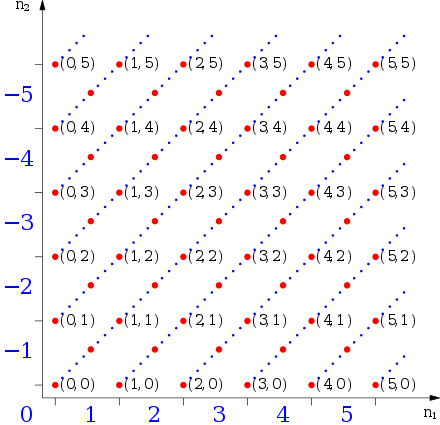
\includegraphics[scale=0.5]{3-set-theory/figs/ndef}
	
	\caption{整数$\Z$的定义}
	\label{fig:zdef}
\end{figure}

\begin{definition}[$\mathbb{Z}$]
一般地, 整数可以定义为: 
  \[
    \mathbb{Z} \triangleq \mathbb{N} \times \mathbb{N}/\sim
  \]
\end{definition}

有了整数, 我们就要为整数定义对应的加法和乘法. 分别记作$+_\Z$和$\times_\Z$. 这样就可以让这个加法和乘法不会因为牵涉了自然数变得``有问题''. 

\begin{definition}[$+_\mathbb{Z}$]
在整数范围的加法定义为: 
  \[
    [(m_1, n_1)] +_{\mathbb{Z}} [(m_2, n_2)] = [m_1 +_{\mathbb{N}} m_2, n_1 +_{\mathbb{N}} n_2]
  \]
\end{definition}

\begin{definition}[$\cdot_\mathbb{Z}$]
在整数范围的乘法定义为: 
  \begin{gather*}
    [(m_1, n_1)] \cdot_{\mathbb{Z}} [(m_2, n_2)] \\
    = [m_1 \cdot_{\mathbb{N}} m_2 +_{\mathbb{N}} n_1 \cdot_{\mathbb{N}} n_2,
       m_1 \cdot_{\mathbb{N}} n_2 +_{\mathbb{N}} n_1 \cdot_{\mathbb{N}} m_2]
  \end{gather*}
\end{definition}

现在我们假设我们的整数已经很好的定义了. 直接沿用其记号, 并且忘记刚刚的所有记号. 接下来我们再定义一个关系$\sim$(和刚刚的内容不一样). 这个关系是定义在$\Z\times (\Z \backslash \set{0_\Z})$上的. 

\begin{definition}
定义一个关系
  \[
    \sim\; \subseteq \mathbb{Z} \times (\mathbb{Z} \setminus \set{0_{\mathbb{Z}}})
  \]
其含义是
  \[
    (a, b) \sim (c, d) \iff a \cdot_{\mathbb{Z}} d = b \cdot_{\mathbb{Z}} c
  \]
\end{definition}

那么请问$\mathbb{Z} \times (\mathbb{Z} \setminus \set{0_{\mathbb{Z}}})/\sim$ 是什么? 


\begin{definition}[$\mathbb{Q}$]
  \[
    \mathbb{Q} \triangleq \mathbb{Z} \times (\mathbb{Z} \setminus \set{0_{\mathbb{Z}}})/\sim
  \]
\end{definition}

\begin{figure}
	\centering
	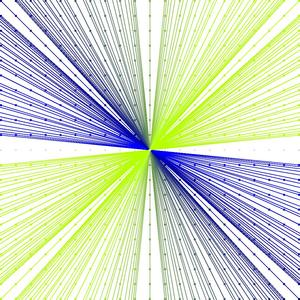
\includegraphics[scale=0.5]{3-set-theory/figs/qdef}
	
	\caption{整数$\Q$的定义}
	\label{fig:zdef}
\end{figure}

如何用有理数定义实数? 请参见《数学分析》Dedekind分割. 

\section{相容关系~--~特殊的二元关系}

如果我们把上一节中的``传递性''去掉, 我们就得到了相容关系. 通俗的讲, 相容关系指的是``如果A和B有这个关系, 那么B和A也有这样的关系''. 也就是二者是``相互作用的''. 例如, 朋友关系. A和B是朋友, 那么B和A也是朋友; 如果A和C是朋友, 我们不一定能够推出B和C也是朋友. 于是我们给出相容关系的定义. 

\begin{definition}[Compatibility relation]
  $R \subseteq X \times X$ is an {\it compatibility relation} on $X$ iff $R$ is
  \begin{itemize}
    \item reflexive: $\forall a \in X.\; a R a$
    \item symmetric: $\forall a, b \in X.\; (a R b \leftrightarrow b R a)$
  \end{itemize}
\end{definition}

\subsection{集合的覆盖}

由于我们通常是对于一个集合来做这样的``相容关系''的定义的, 于是, 我们就希望用一个具体的例子说明这个关系到底在做什么.

\begin{definition}[集合的覆盖(cover)]
	给定非空的集合$A$, 如果
	
	(1) $A_i \subseteq A$并且$A\neq \varnothing$, $i=1,2,3,\cdots,m $;
	
	(2) $\bigcup_{i=1}^m A_i = A$, 
	
	那么称$S$为集合$A$的一个覆盖. 
\end{definition} 

我们可以发现集合的覆盖是不唯一的, 并且我们发现任意一个覆盖, 如果我们把每一个覆盖的$A_i$与他自己做笛卡尔积, 并且最终把它并起来, 事实上就得到了原来的集合的一个相容关系. 

\begin{theorem}
	给定一个集合$A$的一个覆盖$S=\set{A_1 ,A_2 ,\cdots, A_n }$, 有$R=\set{A_1, A_2, \cdots , A_n}$, 则$R=A_1\times A_1 \cup A_2 \times A_2\cup \cdots \cup A_n \times A_n$, 那么我们说$R$是$A$上的相容关系. 
\end{theorem}

\section{函数~--~特殊的二元关系}

\subsection{函数: 作为关系的一个子集}

函数不允许一对多, 这就是它和``关系''最大的去区别. 

回想我们以前学习过的东西, 好像``关系''和方程的图像有点相似. 也就是我们在高中的时候在平面直角坐标系中做的椭圆的图线: $x^2/a^2+y^2/b^2=1(a, b>0)$. 接下来, 我们不妨来看一种特殊的``关系'': 函数. 

\begin{bonus}
    为什么函数不允许``一对多''? 在定义上有什么合理性?
\end{bonus}

让我们重新定义一下以前学过的函数. 

\begin{definition}[Function]
    $f \subseteq A \times B$ is a \red{\it function} \blue{from $A$ to $B$} if

    \[
      \red{\forall} a \in A.\; \red{\exists!} \;b \in B.\; (a, b) \in f.
    \]
\end{definition}

在函数中, 除了定义域和值域之外, 还有陪域. 通常被称作``cod''. 比如对于一个映射(函数)$f: A \to B$, $\dom(f) = A , \purple{\cod}(f) = B$, 对于一个函数的值域$\ran(f) = f(A) \subseteq B$. 

为什么这样定义? 值域为什么不是$B$? 原因是很多时候函数的值域难以求解, 这样就使得我们的表达造成很多不便. 而且很多时候如果强行把$B$当作值域很多时候可能会出现运算不封闭的问题, 在研究某些问题的时候非常不方便. 因此, 我们不妨把这个值域扩大一些, 这样才可以更方便一些. 因此, $B$就叫做``陪域''. 值域只不过是陪域的一个子集. 

对于证明而言, 我们同样有一套形式化的证明语言: 
$\red{\forall a \in A.}, \forall a \in A.\; \exists b \in B. (a, b) \in f, \red{\exists! b \;\in B.}, \forall b, b' \in B.\; (a, b) \in f \land (a, b') \in f \implies b = b'.$

当然我们可以看一些有趣的函数. 

\textbf{1. 恒等函数. } ``恒等''在数学的各个领域里面都是重要的. ``恒等函数''的地位有时候和加法意义下的`0', 乘法意义下的`1'很相似, 其特点是经过一次复合之后还是一样的. 我们一般用$I_X$表示, I的意思是identity的缩写. 其中, 
$$\forall x \in X.\; I_{X}(x) = x.$$

\begin{fun}
    Weierstrass构造了一个处处连续, 处处不可导的函数. 
    $$
    f(x)=\sum_{n=0} ^\infty a^n \cos(b^n \pi x),
    $$
    其中, $0 < a < 1,\; b \text{ is a positive odd integer},\; ab > 1+\frac{3}{2} \pi$. 
\end{fun}

当然, 我们也可以把相似的函数放在一个集合里面. 

\begin{definition}[$Y^{X}$]
    The \red{\it set} of all functions \blue{from $X$ to $Y$}:
    \[
      Y^{X} = \set{f \mid f: X \to Y}
    \]
\end{definition}

举一些例子, $|X|=x, |Y|=y, |Y^X|=x^y$. 

\begin{eg}
    \begin{itemize}
        \item $\forall Y.\; Y^{\emptyset} = \set{\emptyset}$
        \item $\emptyset^{\emptyset} = \set{\emptyset}$
        \item $\forall X \neq \emptyset.\; \emptyset^{X} =  \emptyset$
        \item $2^{X} = \set{0, 1}^{X} \cong \ps{X}$
    \end{itemize}
    
\end{eg}

类似的, 我们可以问: 是否存在由所有函数组成的集合? 像Russell一样, 我们的答案是否定的. 

\begin{theorem}
    There is no set consisting of all functions.
\end{theorem}

\begin{proof}
    Suppose \red{by contradiction} that $A$ is the set of all functions. 
    For every set $X$, there exists a function $I_{\red{\set{X}}}: \set{X} \to \set{X}$.
    \[
      \bigcup_{I_{X} \in A} \dom(I_{X})
        \text{ would be the \purple{universe} that does not exist!}
    \]
\end{proof}

既然函数和集合的结论如此相似, 我们自然地想到函数有没有和集合一样的性质? 

\subsection{作为集合的函数}

\begin{theorem}[函数的外延性原理 (The Principle of Functional Extensionality)]
    
      $f, g$  are functions:
    
    \[
      f = g \iff \dom(f) = \dom(g)
        \land \big(\forall x \in \dom(f).\; f(x) = g(x) \big)
    \]
\end{theorem}

注意定义并没有要求陪域相同, 只要$f = g \iff \forall (a, b).\; ((a, b) \in f \leftrightarrow (a, b) \in g)$满足, 我们就认为这是相等的. 

既然是集合, 我们就要考察一些集合的运算. 如果$f$和$g$是函数, $f \cap g, f \cup g$是函数吗? 因此我们有如下的定理: 

\begin{theorem}[Intersection of Functions]
    \[
      A = \set{x \mid x \in A \cap C \land f(x) = g(x)}
    \]
    \[
      f \cap g = \set{(x, y) \mid x \in A, y = f(x) = g(x)}
    \]
\end{theorem}

\begin{theorem}[Union of Functions]
    {\[
      f \cup g: (A \cup C) \to (B \cup D) \iff
      \forall x \in \dom(f) \cap \dom(g).\; f(x) = g(x)
    \]}
\end{theorem}

举几个例子. 如果我们有$f: \ps{\R} \to \Z$, $f(A) = \left\{\begin{array}{ll}
    \min(A \cap \N) & \text{if } A \cap \N \neq \emptyset \\
      -1 & \text{if } A \cap \N = \emptyset
  \end{array}\right.$. 
注意$\N$的良序原理, $\dom{(f)}\cap \dom{(g)}=\emptyset$. Dichlet函数也可以看作函数的并. 它是$f:\R \to \R$的一个映射. 表达式写做: $D(x) = \left\{\begin{array}{ll}
    1 & \text{if } x \in \Q \\
    0 & \text{if } x \in \R \setminus \Q
\end{array}\right.$注意到这个函数是``处处不连续''的. 

\subsection{特殊函数关系}

有时候函数之间的映射关系也是重要的. 比如, $f:A\to B$, $A$在$B$中的对应元素是不是都是不同的? $B$中的元素有没有全部对应上$A$中的元素(可能不止被对应了一次)? $A$有没有和$B$中元素一一对应? 这样我们就有了单射, 满射的概念. 

\begin{definition}[Injective (one-to-one; 1-1) 单射函数]
    \[
      f: A \to B \qquad {f: A \red{\;\rightarrowtail\;} B}
    \]

    \[
      \forall a_1, a_2 \in A.\; a_1 \neq a_2 \to f(a_1) \neq f(a_2)
    \]
\end{definition}

对于证明而言, 我们可以这样写: $\forall a_1, a_2 \in A.\; f(a_1) = f(a_2) \to a_1 = a_2$. 证明一个函数不是单射函数, 就可以这样写: $\red{\exists} a_1, a_2 \in A.\; a_1 \neq a_2 \land f(a_1) = f(a_2)$. 

\begin{definition}[Surjective (onto) 满射函数]
    \[
      f: A \to B \qquad {f: A \red{\;\twoheadrightarrow\;} B}
    \]
    \[
      \ran(f) = B
    \]
\end{definition}

同样的, 对于证明给定的函数是满射而言, 我们可以这样写: $\forall b \in B. \; \big(\red{\exists} a \in A.\; f(a) = b \big)$, 反之, 我们可以这样写: $\red{\exists} b \in B.\; \big(\red{\forall} a \in A.\; f(a) \neq b \big)$. 

既是双射又是满射的函数一定很特殊, 因为它有一个一一对应的关系. 因此我们给出如下定义: 

\begin{definition}[Bijective (one-to-one correspondence) 双射; 一一对应]
    \[
      f: A \to B \qquad {f: A \red{\;\xleftrightarrow[onto]{1-1}\;} B}
    \]
    \begin{center}
      {1-1 \& onto}
    \end{center}
\end{definition}

那么, 一个集合和它的幂集之间可不可以找到一个满射呢? 其实是不行的. Cantor给出了一个证明.

\begin{theorem}[Cantor Theorem]
    If $f: A \to 2^{A}$, then $f$ is \red{not} onto.
\end{theorem}

\begin{proof}
    Let $A$ be the set and let $f:A\rightarrow 2^A$. To show that $f$ is not onto, we must find $B\in 2^A(i.e. B\subseteq A )$ for which there is no $a\in A$ with no $f(a)=B$. In other words, $B$ is a set that $f$ ``misses''. To this end, let 
    $$
    B={x\in A | x \notin f(x)}
    $$
    We claim there is no $a\in A $ with $f(a)=B$. 
    Suppose, for the sake of contradiction, there is an $a\in A$ such that $f(a)=B$, we pounder: Is $a\in B$?
    \begin{itemize}
        \item if $a\in B$, then, since $B=f(a)$, we have $a\in f(a)$. So by the definition of $B$ , $a\notin f(a)$. that is $a\notin B$. Contradiction!
        \item If $a\notin B=f(a)$, then by the definition of $B$, $a\in B$. Contradiction!  
    \end{itemize} 
    To sum up, it can't be onto. 
\end{proof}

除了反证之外, 还有一个构造性的证明, 我们一并给出. 

\begin{proof}[对角线论证 (Cantor's diagonal argument)]
以下仅适用于可数集合 $A$. 
  \begin{center}
    \begin{tabular}{|c||c|c|c|c|c|c|}
      \hline
      $a$      & \multicolumn{6}{c|}{$f(a)$} \\ \hline
            & 1      & 2      & 3      & 4      & 5      & $\cdots$ \\ \hline \hline
      1      & 1      & 1      & 0      & 0      & 1      & $\cdots$ \\ \hline
      2      & 0      & 0  & 0      & 0      & 0      & $\cdots$ \\ \hline
      3      & 1      & 0      & 0      & 1      & 0      & $\cdots$ \\ \hline
      4      & 1      & 1      & 1      & 0      & 1      & $\cdots$ \\ \hline
      5      & 0      & 1      & 0      & 1      & 0      & $\cdots$ \\ \hline
      $\vdots$ & $\vdots$ & $\vdots$ & $\vdots$ & $\vdots$ & $\vdots$ & $\cdots$ \\ \hline
    \end{tabular}
  \end{center}
\end{proof}

\subsection{作为关系的函数}

\subsubsection{函数的限制}
和关系一样, 函数也有限制等操作. 我们来看看. 

\begin{definition}[Restriction]
  The \red{\it restriction} of a function $f: A \to B$ to $X$
  is the \blue{function}:

  \[
    f|_{X} = \set{(x, y) \in f \mid \purple{x \in X}}
  \]
\end{definition}

注意$X \subseteq A$并不是必要的(虽然平时经常这样用). 

\subsubsection{像和逆像}

\begin{definition}[像 (Image)]
  The \red{\it image} of $X$ under a function $f: A \to B$ is the set
  \[
    {f(X) = \set{y \mid \exists \purple{x \in X}.\; (x, y) \in f}}
  \]
\end{definition}

同样, $X \subseteq \dom(f) = A$也不是必要条件, 尽管通常是这样的. 记号层面, $ f(\set{a}) = \set{b} \quad \text{简记为} \quad f(a) = b$. 

也就是$y \in f(X) \iff \exists x \in X.\; y = f(x)$.

\begin{definition}[逆像 (Inverse Image)]
  The \red{\it inverse image} of $Y$ under a function $f: A \to B$ is the set
  \[
    {f^{-1}(Y) = \set{x \mid \exists \purple{y \in Y}.\; (x, y) \in f}}
  \]
\end{definition}

注意不一定要$Y \subseteq \ran(f)$, 但是很多情况都是满足这样的. 但是注意
\[
    f^{-1}(\set{b}) = \set{a}
      \quad\text{\blue{可简记为}}\quad f^{-1}(b) = \set{a}
      \quad\text{\red{不能简记为}}\quad f^{-1}(b) = a
\]
想一想, 为什么会这样? 

\begin{definition}[逆像 (Inverse Image)]
  The \red{\it inverse image} of $Y$ under a function $f: A \to B$ is the set
  \[
    {f^{-1}(Y) = \set{x \mid \exists \purple{y \in Y}.\; (x, y) \in f}}
  \]
\end{definition}

这样一来, 我们就有这样的关系 :$y \in f(X) \iff \exists x \in X.\; y = f(x), x \in f^{-1}(Y) \iff f(x) \in Y$. 

需要注意的是, 如果有$f: a\rightarrow b$, $a \in A_{0} \red{\;\centernot\implies\;} f(a) \in f(A_{0})$, 这个式子才可以成立: $a \in A_{0} \purple{\;\cap\; A} \blue{\;\implies\;} f(a) \in f(A_{0})$.

关于求逆也有很多的性质. 很多时候我们可能会想当然的误用. 所以使用之前一定要小心, 小心, 再小心. 

幸运的是, 它还保留有很多性质. 我们一一罗列, 并给出一些证明. 

\begin{theorem}[Properties of $f$ and $f^{-1}$]
  \[
    f: A \to B \qquad
    {A_1, A_2 \subseteq A,\; B_1, B_2 \subseteq B}
  \]

  \begin{enumerate}
    \item \purple{$f$ preserves only $\subseteq$ and $\cup$:}
      \begin{enumerate}
        \item $A_1 \subseteq A_2 \implies f(A_1) \subseteq f(A_2)$
        \item \teal{$f(A_1 \cup A_2) = f(A_1) \cup f(A_2)$}
        \item $f(A_1 \cap A_2) \subseteq f(A_1) \cap f(A_2)$
        \item $f(A_1 \setminus A_2) \supseteq f(A_1) \setminus f(A_2)$
      \end{enumerate}
    \item \purple{$f^{-1}$ preserves $\subseteq$, $\cup$, $\cap$, and $\setminus$:}\begin{enumerate}
      \item $B_1 \subseteq B_2 \implies f^{-1}(B_1) \subseteq f^{-1}(B_2)$
      \item \teal{$f^{-1}(B_1 \cup B_2) = f^{-1}(B_1) \cup f^{-1}(B_2)$}
      \item $f^{-1}(B_1 \cap B_2) = f^{-1}(B_1) \cap f^{-1}(B_2)$
      \item \teal{$f^{-1}(B_1 \setminus B_2) = f^{-1}(B_1) \setminus f^{-1}(B_2)$}
    \end{enumerate}
  \end{enumerate}
\end{theorem}

对于$A_1 \subseteq A_2 \implies f(A_1) \subseteq f(A_2)$, 证明如下: 

\begin{proof}
  \setcounter{equation}{0}
  \begin{align*}
    &b \in f(A_{1}) \\
    \iff & \exists a \in A_{1}.\; b = f(a) \\
    \red{\implies} & \exists a \in A_{2}.\; b = f(a) \\
    \iff & b \in f(A_{2})
  \end{align*}
\end{proof}

对于$f(A_1 \cap A_2) \red{\;\subseteq\;} f(A_1) \cap f(A_2)$, 证明如下. 注意是哪一步变换, 使得它的箭头方向变为单向了, 为什么? 

\begin{proof}
  \red{对任意 $b$,}
  \setcounter{equation}{0}
  \begin{align*}
    &b \in f(A_1 \cap A_2) \\[6pt]
    \iff & \exists a \in A_1 \cap A_2.\; b = f(a) \\
    \red{\implies}& \big(\exists a \in A_{1}.\; b = f(a)\big)
      \land \big(\exists a \in A_{2}.\; b = f(a)\big) \\
    \iff & b \in f(A_{1}) \land b = f(A_{2}) \\
    \iff & b \in f(A_1) \cap f(A_2)
  \end{align*}
\end{proof}

对于$f(A_1 \setminus A_2) \red{\;\supseteq\;} f(A_1) \setminus f(A_2)$ : 

\begin{proof}
  \red{对任意 $b$,}
  \setcounter{equation}{0}
  \begin{align*}
    &b \in f(A_{1}) \setminus f(A_{2}) \\[6pt]
    \iff & b \in f(A_{1}) \land b \notin f(A_{2}) \\
    \iff & (\exists a_{1} \in A_{1}.\; b = f(a_{1})) \land
      (\forall a_{2} \in A_{2}.\; b \neq f(a_{2})) \\
    \red{\implies} & \exists a \in A_{1} \setminus A_{2}.\; b = f(a) \\
    \iff & b \in f(A_{1} \setminus A_{2})
  \end{align*}
\end{proof}

对于$B_1 \subseteq B_2 \implies f^{-1}(B_1) \subseteq f^{-1}(B_2)$, 证明如下:

\begin{proof}
  \red{对任意 $a$,}
  \setcounter{equation}{0}
  \begin{align*}
    &a \in f^{-1}(B_{1}) \\
    \iff & f(a) \in B_{1} \\
    \red{\implies} & f(a) \in B_{2} \\[6pt]
    \iff & a \in f^{-1}(B_{2})
  \end{align*}
\end{proof}

对于$f^{-1}(B_1 \cap B_2) = f^{-1}(B_1) \cap f^{-1}(B_2)$, 证明如下: 

\begin{proof}
  \red{对任意 $a$,}
  \setcounter{equation}{0}
  \begin{align*}
    &a \in f^{-1}(B_{1} \cap B_{2}) \\
    \iff & f(a) \in B_{1} \cap B_{2} \\
    \iff & f(a) \in B_{1} \land f(a) \in B_{2} \\
    \iff & a \in f^{-1}(B_{1}) \land a \in f^{-1}(B_{2}) \\
    \iff & a \in f^{-1}(B_{1}) \cap f^{-1}(B_{2})
  \end{align*}
\end{proof}

对于$A_0 \subseteq A \implies A_0 \subseteq f^{-1}(f(A_0))$, 有
\begin{proof}
  \red{对任意 $b$,}
  \setcounter{equation}{0}
  \begin{align*}
    &a \in A_{0} \\
    \implies & a \in A_{0} \purple{\;\cap\; A} \\
    \red{\implies} & f(a) \in f(A_{0}) \\
    \iff & a \in f^{-1}(f(A_{0}))
  \end{align*}
\end{proof}

对于$B_0 \supseteq f(f^{-1}(B_0))$, 思考什么时候这个条件是充要的($\iff$)?

\begin{proof}
  \red{对任意 $b$,}
  \setcounter{equation}{0}
  \begin{align*}
    &b \in f(f^{-1}(B_0)) \\
    \iff & \exists a \in f^{-1}(B_0).\; b = f(a) \\[6pt]
    \iff & \exists a \in A.\; f(a) \in B_0 \land b = f(a) \\[6pt]
    \red{\implies} & b \in B_0
  \end{align*}
  ``iff'' when $f$ is surjective and $$B_0 \subseteq \ran(f)$$.
\end{proof}

\subsubsection{函数的复合}
作为化简单为复杂的利器, 和关系一样, 函数也有复合. 

\begin{definition}[Composition]
  \[
    f: A \to B \qquad g: C \to D
  \]
  \[
    \red{\ran(f) \subseteq C}
  \]

  The \red{\it composite function} \blue{$g \circ f: A \to D$} is defined as

  \[
    (g \circ f) (x) = g(f(x))
  \]
\end{definition}

\begin{bonus}
  回顾关系复合的定义: 
  The {\it composition} of relations $R$ and $S$ is the relation
    \[
      R \circ S = \set{(a, c) \mid \red{\exists b}: (a, b) \in S \land (b, c) \in R}
    \]

  和函数的有什么不同? 为什么是存在? 
\end{bonus}

\begin{theorem}[Associative Property for Composition]
  \[
    f: A \to B \quad g: B \to C \quad h: C \to D
  \]

  \[
    h \circ (g \circ f) = (h \circ g) \circ f
  \]
\end{theorem}

\begin{proof}
  我们只需证明: 
  \begin{enumerate}
    \item
      \[
        \dom(h \circ (g \circ f)) = \dom((h \circ g) \circ f)
      \]
    \item
      \[
        \forall x \in A.\; (h \circ (g \circ f))(x) = ((h \circ g) \circ f)(x)
      \]
  \end{enumerate}


对于$(h \circ (g \circ f))(x) = ((h \circ g) \circ f)(x)$:


  \setcounter{equation}{0}
      \begin{align*}
        &(h \circ (g \circ f))(x) \\[6pt]
        =\; &h((g \circ f) (x)) \\[6pt]
        =\; &h(g(f(x)))
      \end{align*}
      \setcounter{equation}{0}
      \begin{align*}
        &((h \circ g) \circ f)(x) \\[6pt]
        =\; &((h \circ g) (f(x))) \\[6pt]
        =\; &h(g(f(x)))
      \end{align*}
\end{proof}

\begin{theorem}
  $f: A \to B \qquad g: B \to C$, 
  \begin{itemize}
    \item If $f, g$ are injective, then $g \circ f$ is injective.
    \item \teal{If $f, g$ are surjective, then $g \circ f$ is surjective.}
    \item If $f, g$ are bijective, then $g \circ f$ is bijective.
  \end{itemize}
\end{theorem}

对于第一条, 我们写出``injective''的定义, 然后完成逻辑推演. 

\begin{proof}
  $$\forall a_1, a_2 \in A.\;
      \Big( (g \circ f)(a_1) = (g \circ f)(a_2) \to a_1 = a_2 \Big)$$

      \begin{align*}
        &(g \circ f)(a_1) = (g \circ f)(a_2) \\
        \iff &g(f(a_{1})) = g(f(a_{2})) \\[6pt]
        \implies &f(a_{1}) = f(a_{2}) \\[6pt]
        \implies &a_{1} = a_{2}
      \end{align*}


\end{proof}

对于第二条, 我们写出``surjective''的定义. 


\begin{proof}
  $$\forall c \in C.\; \Big( \exists a \in A.\; (g \circ f)(a) = c \Big)$$
\end{proof}

对于第三条, 如出一辙. 

\begin{proof}
  \red{对任意 $a_{1}, a_{2}$,}
  \setcounter{equation}{0}
  \begin{align*}
    &f(a_{1}) = f(a_{2}) \\
    \implies & g(f(a_{1})) = g(f(a_{2})) \\
    \implies & (g \circ f) (a_{1}) = (g \circ f) (a_{2}) \\[6pt]
    \implies & a_{1} = a_{2}
  \end{align*}
\end{proof}

\begin{theorem}[]
  \[
    f: A \to B \qquad g: B \to C
  \]

  \begin{enumerate}
    \item \teal{If $g \circ f$ is injective, then $f$ is injective.}
    \item If $g \circ f$ is surjective, then $g$ is surjective.
  \end{enumerate}
\end{theorem}
因为(1)和(2)很像, 因此只证明(2). 注意充要条件是在哪一步消失的. 
\begin{proof}
  \red{对任意 $a_{1}, a_{2}$,}
  \setcounter{equation}{0}
  \begin{align*}
    & g \circ f \text{ is surjective}\\
    \iff & \forall c \in C.\; \exists a \in A.\; (g \circ f)(a) = c \\
    \iff & \forall c \in C.\; \exists a \in A.\; g(f(a)) = c \\
    \red{\implies} & \forall c \in C.\; \exists b \in B.\; g(b) = c \\
    \iff & g \text{ is surjective}
  \end{align*}
\end{proof}

\subsubsection{反函数}

什么时候有反函数? 反函数具有哪些性质? 在高中的时候老师可能不会和我们讲, 现在我们来探索一下反函数的性质. 

\begin{definition}[反函数 (Inverse Function)]
  Let $f: A \to B$ be a function. 

  The \red{\it inverse} of $f$ is a \teal{function}
  from $B$ to $A$, denoted \blue{$f^{-1}: B \to A$} \\
  if $f$ is bijective. \\

  We call $f^{-1}$ \blue{the} \red{\it inverse function} of $f$.
\end{definition}


\begin{definition}[Invertible]
      $f: X \to Y$ is {\it invertible} if there exists $g: Y \to X$ such that
  
      \[
        f(x) = y \iff g(y) = x.
      \]
\end{definition}

下面这个定理展示了什么时候具有反函数. 
\begin{theorem}
  $f$ is invertible $\iff$ $f$ is bijective.
\end{theorem}

\begin{theorem}
  Suppose that $f: A \to B$ is bijective.
  Then, its inverse function $f^{-1}: B \to A$ is unique.
\end{theorem}

\begin{proof}
  By contradiction. Omitted.
\end{proof}

\begin{theorem}[]
  \[
    \red{\boxed{f: A \to B \text{ is bijective}}}
  \]

  \begin{enumerate}
    \item $f \circ f^{-1} = I_B$
    \item $f^{-1} \circ f = I_A$
    \vspace{0.30cm}
    \item \teal{$f^{-1} \text{ is bijective}$}
    \vspace{0.30cm}
    \item $g: B \to A \land f \circ g = I_B \implies g = f^{-1}$
    \item $g: B \to A \land g \circ f = I_A \implies g = f^{-1}$
  \end{enumerate}
\end{theorem}

这些定理是帮助我们找到反函数/说明反函数不存在的一些好的结论.

对于(1). 
\begin{proof}
  \red{对任意 $b \in B$,}
  \[
    (f \circ f^{-1})(b) = f(f^{-1}(b))
  \]

    Suppose that $a = f^{-1}(b)$
    \[
      \red{\boxed{a = f^{-1}(b) \iff f(a) = b}}
    \]
    \[
    (f \circ f^{-1})(b) = f(f^{-1}(b)) = \red{f(a)} = b
  \]
\end{proof}

对于(2).
\begin{proof}
  $g = \purple{(f^{-1} \circ f) \circ g = f^{-1} \circ (f \circ g) = f^{-1} \circ I_B} = f^{-1}$
\end{proof}

我们当然可以看一看反函数的复合是怎样的一个情况. \footnote{理由不充分, 需要补充证明}

\begin{theorem}[Inverse of Composition]
  \[
    \text{Both } f: A \to B \text{ and } g: B \to C \text{ are bijective}
  \]

  \begin{enumerate}
    \item $g \circ f \text{ is bijective}$
    \item $(g \circ f)^{-1} = f^{-1} \circ g^{-1}$
    \item $f \circ g = I_B \land g \circ f = I_A \implies g = f^{-1}$
  \end{enumerate}
\end{theorem}

那么, 我们就从集合论的角度构建了我们高中学习过的内容. 

\section{序关系}

我们在本章的开头介绍关系的时候就提到了``偏序''以及``全序''. 下面我们来通过一些更多的例子好好体会一下这些``序关系''带给我们的思维上的碰撞, 并且我们会重新看一看定义极限的$\epsilon-\delta$语言里面的重要关系: $<$(小于号), 为什么换成$(\leq)$(小于等于)就不行了. 并且这件事情能够让我们理解什么叫``开'', 什么叫``闭''; 同时也对于高等数学课程中空间解析几何的内容有一个更自然的想法. 

